\begin{figure}[H]
    \centering
    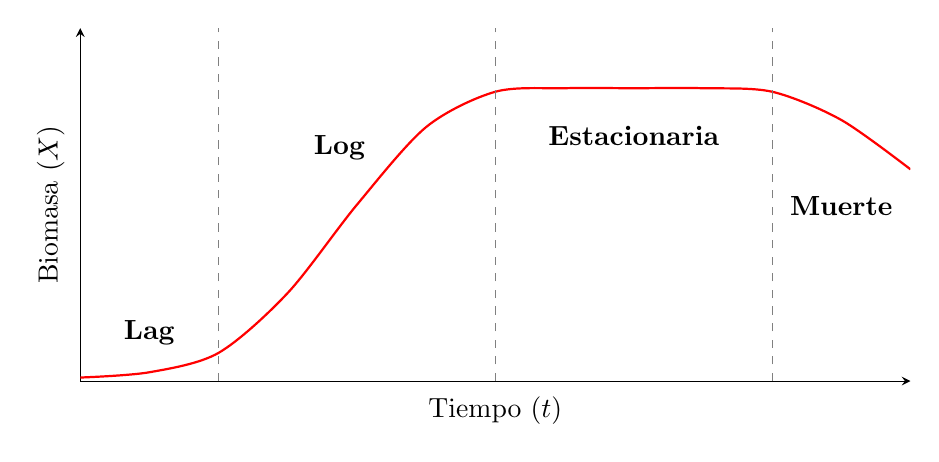
\begin{tikzpicture}
        \begin{axis}[
            width=\linewidth,
            height=0.5\linewidth,
            axis lines = left,
            xlabel = Tiempo ($t$),
            xmin=0, xmax=24,
            xtick=\empty,
            ylabel = Biomasa ($X$),
            ymin=0, ymax=10,
            ytick=\empty,
            grid=major,
            grid style={dashed, gray!20},
        ]
        \addplot[thick, red, smooth, tension=0.5] coordinates {
            (0, 0.1)      % Inoculación
            (2, 0.25)     % Fase lag
            (4, 0.8)
            (6, 2.5)
            (8, 5)      % Inicio fase log
            (10, 7.2)
            (12, 8.2)     % Mitad fase log
            (14, 8.3)
            (16, 8.3)     % Fin fase log
            (18, 8.3)     % Fase estacionaria
            (20, 8.2)
            (22, 7.4)     % Fase muerte
            (24, 6)
        };
        \draw[dashed, gray] (4,0) -- (4,10);
        \draw[dashed, gray] (12,0) -- (12,10);
        \draw[dashed, gray] (20,0) -- (20,10);
        \node[anchor=north] at (2,2) {\textbf{Lag}};
        \node[anchor=north] at (7.5,7.25) {\textbf{Log}};
        \node[anchor=north] at (16,7.5) {\textbf{Estacionaria}};
        \node[anchor=north] at (22,5.5) {\textbf{Muerte}};
        \end{axis}
    \end{tikzpicture}
    
    \rule{\linewidth}{0.2pt}
    \caption{Ejemplo de curva de crecimiento bacteriano}
    \label{fig:curva_crecimiento_bacteriano}
\end{figure}